\section{Local convergence}
Following~\cite{r1}, GAN training can be formulated as a dynamical system where the update operator is given by $F_h(\theta,\psi)=(\theta,\psi)+hv(\theta,\psi)$. $h$ is the learning rate and $v$ denotes the gradient vector field:
\begin{equation}
v(\theta,\psi)=\begin{pmatrix}
 -\nabla_\theta\mathcal{L}(\theta,\psi) \\
 \nabla_\psi\mathcal{L}(\theta,\psi)
\end{pmatrix}
\end{equation}
Mescheder et al.~\cite{gannum} showed that local convergence near $(\theta^*,\psi^*)$ can be analyzed by examining the spectrum of the Jacobian $\textbf{J}_{F_h}$ at the equilibrium: if the Jacobian has eigenvalues with absolute value bigger than 1, then training does not converge. On the other hand, if all eigenvalues have absolute value smaller than 1, then training will converge to $(\theta^*,\psi^*)$ at a linear rate. If all eigenvalues have absolute value equal to 1, the convergence behavior is undetermined.

Given some calculations~\cite{r1}, we can show that the eigenvalues of the Jacobian of the update operator $\lambda_{\textbf{J}_{F_h}}$ can be determined by $\lambda_{\textbf{J}_v}$:
\begin{equation}
\lambda_{\textbf{J}_{F_h}}=1+h\lambda_{\textbf{J}_v}\ .
\end{equation}
That is, given small enough $h$~\cite{r1}, the training dynamics can instead be examined using $\lambda_{\textbf{J}_v}$,~\ie, the eigenvalues of the Jacobian of the gradient vector field. If all $\lambda_{\textbf{J}_v}$ have a negative real part, the training will locally converge to $(\theta^*,\psi^*)$ at a linear rate. On the other hand, if some $\lambda_{\textbf{J}_v}$ have a positive real part, the training is not convergent. If all $\lambda_{\textbf{J}_v}$ have a zero real part, the convergence behavior is inconclusive.

\section{DiracRpGAN: A demonstration of non-convergence}
\paragraph{Summary.} To obtain DiracRpGAN, we apply Eq.~\ref{eq:rpgan} to the DiracGAN~\cite{r1} problem setting. After simplification, DiracRpGAN and DiracGAN are different only by a constant. They have the same gradient vector field, therefore all proofs are identical to Mescheder~\etal~\cite{r1}.

\paragraph{Definition B.1.} \emph{The DiracRpGAN consists of a (univariate) generator distribution $p_{\theta} = \delta_{\theta}$ and a linear discriminator $D_{\psi}(x) = \psi \cdot x$. The true data distribution $p_{\mathcal{D}}$ is given by a Dirac distribution concentrated at 0.}

In this setup, the RpGAN training objective is given by:
\begin{equation}
\label{eq:diracrpgan}
    \mathcal{L}(\theta, \psi) = f(\psi \theta)\ .
\end{equation}
We can now show analytically that DiracRpGAN does not converge without regularzation.

\paragraph{Lemma B.2.} \emph{The unique equilibrium point of the training objective in Eq.~\ref{eq:diracrpgan} is given by $\theta = \psi = 0$. Moreover, the Jacobian of the gradient vector field at the equilibrium point has the two eigenvalues $\pm f'(0)i$ which are both on the imaginary axis.}

The gradient vector field $v$ of Eq.~\ref{eq:diracrpgan} is given by:
\begin{equation}
    v(\theta, \psi) =
    \begin{pmatrix}
    -\nabla_{\theta} \mathcal{L}(\theta, \psi) \\
    \nabla_{\psi} \mathcal{L}(\theta, \psi)
    \end{pmatrix} =
    \begin{pmatrix}
    -\psi f'(\psi \theta) \\
    \theta f'(\psi \theta)
    \end{pmatrix}
\end{equation}
and the Jacobian of $v$:
\begin{equation}
    \textbf{J}_v =
    \begin{pmatrix}
    -\psi^2 f''(\psi\theta) & -f'(\psi\theta) - \psi\theta f''(\psi\theta) \\
    f'(\psi\theta) + \psi\theta f''(\psi\theta) & \theta^2 f''(\psi\theta)
    \end{pmatrix}
\end{equation}
Evaluating $\textbf{J}_v$ at the equilibrium point $\theta = \psi = 0$ gives us:
\begin{equation}
    \textbf{J}_v \biggr\rvert_{(0,0)} =
    \begin{pmatrix}
    0 & -f'(0) \\
    f'(0) & 0
    \end{pmatrix}
\end{equation}
Therefore, the eigenvalues of $\textbf{J}_v$ are $\lambda_{1/2} = \pm f'(0) i$, both of which have a real part of 0. Thus, the convergence of DiracRpGAN is inconclusive and further analysis is required.

\paragraph{Lemma B.3.} \emph{The integral curves of the gradient vector field $v(\theta, \psi)$ do not converge to the equilibrium point. More specifically, every integral curve $(\theta(t), \psi(t))$ of the gradient vector field $v(\theta, \psi)$ satisfies $\theta(t)^2 + \psi(t)^2 = const$ for all $t \in [0, \infty)$.}

Let $R(\theta, \psi) = \frac{1}{2} (\theta^2 + \psi^2)$, then:
\begin{align}
    \frac{\mathrm{d}}{\mathrm{d}t} R(\theta(t), \psi(t)) \nonumber &= -\theta(t) \psi(t) f'(\theta(t) \psi(t)) + \psi(t) \theta(t) f'(\theta(t) \psi(t)) \nonumber \\
    &= 0\ .
\end{align}
We see that the distance between $(\theta, \psi)$ and the equilibrium point $(0,0)$ stays constant. Therefore, training runs in circles and never converges.

Next, we investigate the convergence behavior of DiracRpGAN with regularization. For DiracRpGAN, both $R_1$ and $R_2$ can be reduced to the following form:
\begin{equation}
    R(\psi) = \frac{\gamma}{2} \psi^2
\end{equation}

\paragraph{Lemma B.4.} \emph{The eigenvalues of the Jacobian of the gradient vector field for the gradient-regularized DiracRpGAN at the equilibrium point are given by
\begin{equation}
\label{eq:ev}
    \lambda_{1/2} = -\frac{\gamma}{2} \pm \sqrt{\frac{\gamma^2}{4}-f'(0)}
\end{equation}
In particular, for $\gamma > 0$ all eigenvalues have a negative real part. Hence, gradient descent is locally convergent for small enough learning rates.}

With regularization, the gradient vector field becomes
\begin{equation}
    \Tilde{v} (\theta, \psi) =
    \begin{pmatrix}
        -\psi f'(\psi\theta) \\
        \theta f'(\psi\theta) - \gamma\psi
    \end{pmatrix}
\end{equation}
the Jacobian of $\Tilde{v}$ is then given by
\begin{equation}
    \textbf{J}_{\Tilde{v}} =
    \begin{pmatrix}
    -\psi^2 f''(\psi\theta) & -f'(\psi\theta) - \psi\theta f''(\psi\theta) \\
    f'(\psi\theta) + \psi\theta f''(\psi\theta) & \theta^2 f''(\psi\theta) - \gamma
    \end{pmatrix}
\end{equation}
evaluating the Jacobian at $\theta = \psi = 0$ yields
\begin{equation}
    \textbf{J}_{\Tilde{v}} \biggr\rvert_{(0, 0)} =
    \begin{pmatrix}
        0 & -f'(0) \\
        f'(0) & -\gamma
    \end{pmatrix}
\end{equation}
given some calculations, we arrive at Eq.\ref{eq:ev}.

\section{General Convergence Results}
\paragraph{Summary.} The proofs are largely the same as Mescheder~\etal~\cite{r1}. We use the same proving techniques, and only slightly modify the assumptions and proof details to adapt Mescheder~\etal's effort to RpGAN. Like in~\cite{r1}, our proofs do not rely on unrealistic assumptions such as $\supp p_\mathcal{D}=\supp p_\theta$.

\subsection{Assumptions}
We closely follow~\cite{r1} but modify the assumptions wherever necessary to tailor the proofs for RpGAN. Like in~\cite{r1}, we also consider the realizable case where there exists $\theta$ such that $G_\theta$ produces the true data distribution.

\paragraph{Assumption~\upperRomannumeral{1}.}
\label{a:1}
\emph{We have $p_{\theta^*}=p_\mathcal{D}$, and $D_{\psi^*}=C$ in some local neighborhood of $\supp p_\mathcal{D}$, where $C$ is some arbitrary constant.}

\noindent Since RpGAN is defined on critic difference rather than raw logits, we no longer require $D_{\psi^*}$ to produce 0 on $\supp p_\mathcal{D}$, instead any constant $C$ would suffice.

\paragraph{Assumption~\upperRomannumeral{2}.}
\label{a:2}
\emph{We have $f^\prime(0)\neq0$ and $f^{\prime\prime}(0)<0$.}

\noindent This assumption is the same as in~\cite{r1}. The choice $f(t) = -\log(1+e^{-t})$ adopted in the main text satisfies this assumption.

As discussed in~\cite{r1}, there generally is not a single equilibrium point $(\theta^*,\psi^*)$, but a submanifold of equivalent equilibria corresponding to different parameterizations of the same function. It is therefore necessary to represent the equilibrium as \emph{reparameterization manifolds} $\mathcal{M}_G$ and $\mathcal{M}_D$. We modify the reparameterization $h$ as follows:
\begin{equation}
\label{eq:h}
h(\psi)=\mathbb{E}_{\substack{x\sim p_\mathcal{D}\\y\sim p_\mathcal{D}}}\left[\left | D_\psi(x)-D_\psi(y)\right |^2   +  \left \| \nabla_x D_\psi(x) \right \|^2\right]
\end{equation}
to account for the fact that $D_{\psi^*}$ is now allowed to have any constant value on $\supp p_\mathcal{D}$. The \emph{reparameterization manifolds} are then given by:
\begin{align}
&\mathcal{M}_G=\{\theta\,\rvert\,p_\theta=p_\mathcal{D}\} \\
&\mathcal{M}_D=\{\psi\,\rvert\,h(\psi)=0 \}
\end{align}
We assume the same regularity properties as in~\cite{r1} for $\mathcal{M}_G$ and $\mathcal{M}_D$ near the equilibrium. To state these assumptions, we need:
\begin{equation}
g(\theta)=\mathbb{E}_{x\sim p_\theta}\left[\nabla_\psi D_\psi\rvert_{\psi=\psi^*}\right]
\end{equation}
which leads to:
\paragraph{Assumption~\upperRomannumeral{3}.}
\label{a:3}
\emph{There are $\epsilon$-balls $B_\epsilon(\theta^*)$ and $B_\epsilon(\psi^*)$ around $\theta^*$ and $\psi^*$ so that $\mathcal{M}_G\,\cap\,B_\epsilon(\theta^*)$ and $\mathcal{M}_D\,\cap\,B_\epsilon(\psi^*)$ define $\mathcal{C}^1$-manifolds. Moreover, the following holds}:
\begin{enumerate}[label=(\roman*)]
\item \emph{if $v\in\mathbb{R}^n$ is not in $\mathcal{T}_{\psi^*}\mathcal{M}_D$, then $\partial_v^2h(\psi^*)\neq0$}.
\item \emph{if $w\in\mathbb{R}^m$ is not in $\mathcal{T}_{\theta^*}\mathcal{M}_G$, then $\partial_wg(\theta^*)\neq0$}.
\end{enumerate}

These two conditions have exactly the same meanings as in~\cite{r1}: the first condition indicates the geometry of $\mathcal{M}_D$ can be locally described by the second derivative of $h$. The second condition implies that $D$ is strong enough that it can detect any deviation from the equilibrium generator distribution. This is the only assumption we have about the expressiveness of $D$.

\subsection{Convergence}
We can now show the general convergence result for gradient penalized RpGAN, consider the gradient vector field with either $R_1$ or $R_2$ regularization:
\begin{equation}
\label{eq:vreg}
\tilde{v}_i(\theta,\psi)=\begin{pmatrix}
-\nabla_\theta\mathcal{L}(\theta,\psi)\\ 
\nabla_\psi\mathcal{L}(\theta,\psi)-\nabla_\psi R_i(\theta,\psi)
\end{pmatrix}
\end{equation}
note that the convergence result can also be trivially extended to the case where both $R_1$ and $R_2$ are applied. We omit the proof for this case as it is redundant once the convergence with either regularization is proven.

\paragraph{Theorem.} \emph{Assume Assumption~\upperRomannumeral{1},~\upperRomannumeral{2} and~~\upperRomannumeral{3} hold for $(\theta^*,\psi^*)$. For small enough learning rates, gradient descent for $\tilde{v}_1$ and $\tilde{v}_2$ are both convergent to $\mathcal{M}_G\times\mathcal{M}_D$ in a neighborhood of $(\theta^*,\psi^*)$. Moreover, the rate of convergence is at least linear}.

We extend the convergence proof by Mescheder~\etal~\cite{r1} to our setting. We first prove lemmas necessary to our main proof.

\paragraph{Lemma C.2.1.} \emph{Assume $J\in\mathbb{R}^{(n+m)\times(n+m)}$ is of the following form}:
\begin{equation}
J=\begin{pmatrix}
0 & -B^\top\\ 
B & -Q
\end{pmatrix}
\end{equation}
\emph{where $Q\in\mathbb{R}^{m\times m}$ is a symmetric positive definite matrix and $B\in\mathbb{R}^{m\times n}$ has full column rank. Then all eigenvalues $\lambda$ of $J$ satisfy $\Re(\lambda)< 0$}.

\emph{Proof.} See Mescheder~\etal~\cite{r1}, Theorem A.7.

\paragraph{Lemma C.2.2.} \emph{The gradient of $\mathcal{L}(\theta,\psi)$~\wrt $\theta$ and $\psi$ are given by}:
\begin{align}
&\nabla_\theta\mathcal{L}(\theta,\psi)=\mathbb{E}_{\substack{z\sim p_z\\x\sim p_\mathcal{D}}}[f^\prime(D_\psi(G_\theta(z))-D_\psi(x)) \left[\nabla_\theta G_\theta(z)\right]^\top\nabla_xD_\psi(G_\theta(z))] \\
\label{grad_psi}
&\nabla_\psi\mathcal{L}(\theta,\psi)=\mathbb{E}_{\substack{z\sim p_z\\x\sim p_\mathcal{D}}}[f^\prime(D_\psi(G_\theta(z))-D_\psi(x)) (\nabla_\psi D_\psi(G_\theta(z))-\nabla_\psi D_\psi(x))]
\end{align}
\emph{Proof.} This is just the chain rule.

\paragraph{Lemma C.2.3.} \emph{Assume that $(\theta^*,\psi^*)$ satisfies Assumption~\upperRomannumeral{1}. The Jacobian of the gradient vector field $v(\theta,\psi)$ at $(\theta^*,\psi^*)$ is then}
\begin{equation}
\textbf{J}_v\biggr\rvert_{(\theta^*,\psi^*)}=\begin{pmatrix}
0 & -K^\top_{DG}\\ 
K_{DG} & K_{DD}
\end{pmatrix}
\end{equation}
\emph{the terms $K_{DD}$ and $K_{DG}$ are given by}
\begin{align}
\label{kdd}
&K_{DD}=f^{\prime\prime}(0)\mathbb{E}_{\substack{x\sim p_\mathcal{D}\\y\sim p_\mathcal{D}}}[(\nabla_\psi D_{\psi^*}(x)-\nabla_\psi D_{\psi^*}(y))(\nabla_\psi D_{\psi^*}(x)-\nabla_\psi D_{\psi^*}(y))^\top] \\
\label{kdg}
&K_{DG}=f^\prime(0)\nabla_\theta\mathbb{E}_{x\sim p_\theta}[\nabla_\psi D_{\psi^*}(x)]\,\rvert_{\theta=\theta^*}
\end{align}

\emph{Proof.} Note that
\begin{equation}
\textbf{J}_v\biggr\rvert_{(\theta^*,\psi^*)}=\begin{pmatrix}
-\nabla^2_\theta\mathcal{L}(\theta^*,\psi^*) & -\nabla^2_{\theta,\psi}\mathcal{L}(\theta^*,\psi^*) \\ 
\nabla^2_{\theta,\psi}\mathcal{L}(\theta^*,\psi^*) & \nabla^2_\psi\mathcal{L}(\theta^*,\psi^*)
\end{pmatrix}
\end{equation}
By Assumption~\upperRomannumeral{1}, $D_{\psi^*}=C$ in some neighborhood of $\supp p_\mathcal{D}$. Therefore we also have $\nabla_x D_{\psi^*}=0$ and $\nabla^2_x D_{\psi^*}=0$ for $x\in\supp p_\mathcal{D}$. Using these two conditions, we see that $\nabla^2_\theta\mathcal{L}(\theta^*,\psi^*)=0$.

To see Eq.\ref{kdd} and Eq.\ref{kdg}, simply take the derivatives of Eq.\ref{grad_psi} and evaluate at $(\theta^*,\psi^*)$.

\paragraph{Lemma C.2.4.} \emph{The gradient $\nabla_\psi R_i(\theta,\psi)$ of the regularization terms $R_i$, $i\in\{1,2\}$,~\wrt $\psi$ are}
\begin{align}
&\nabla_\psi R_1(\theta,\psi)=\gamma\mathbb{E}_{x\sim p_\mathcal{D}}[\nabla_{\psi,x}D_\psi\nabla_xD_\psi] \\
&\nabla_\psi R_2(\theta,\psi)=\gamma\mathbb{E}_{x\sim p_\theta}[\nabla_{\psi,x}D_\psi\nabla_xD_\psi]
\end{align}

\emph{Proof.} See Mescheder~\etal~\cite{r1}, Lemma D.3.

\paragraph{Lemma C.2.5.} \emph{The second derivatives $\nabla^2_\psi R_i(\theta^*,\psi^*)$ of the regularization terms $R_i$, $i\in\{1,2\}$,~\wrt $\psi$ at $(\theta^*,\psi^*)$ are both given by}
\begin{equation}
L_{DD}=\gamma\mathbb{E}_{x\sim p_\mathcal{D}}[AA^\top]
\end{equation}
\emph{where $A=\nabla_{\psi,x}D_{\psi^*}$. Moreover, both regularization terms satisfy $\nabla_{\theta,\psi}R_i(\theta^*,\psi^*)=0$.}

\emph{Proof.} See Mescheder~\etal~\cite{r1}, Lemma D.4.

Given Lemma C.2.3, Lemma C.2.5 and Eq.\ref{eq:vreg}, we can now show that the Jacobian of the regularized gradient field at the equilibrium point is given by
\begin{equation}
\textbf{J}_{\tilde{v}}\biggr\vert_{(\theta^*,\psi^*)}=\begin{pmatrix}
0 & -K_{DG}^\top\\ 
K_{DG} & M_{DD}
\end{pmatrix}
\end{equation}
where $M_{DD}=K_{DD}-L_{DD}$. To prove our main theorem, we need to examine $\textbf{J}_{\tilde{v}}$ when restricting it to the space orthogonal to $\mathcal{T}_{(\theta^*,\psi^*)}\mathcal{M}_G\times\mathcal{M}_D$.

\paragraph{Lemma C.2.6.} \emph{Assume Assumptions~\upperRomannumeral{2} and~\upperRomannumeral{3} hold. If $v\neq0$ is not in $\mathcal{T}_{\psi^*}\mathcal{M}_D$, then $v^\top M_{DD}v<0$.}

\emph{Proof.} By Lemma C.2.3 and Lemma C.2.5, we have
\begin{align}
&v^\top K_{DD}v=f^{\prime\prime}(0)\mathbb{E}_{\substack{x\sim p_\mathcal{D}\\y\sim p_\mathcal{D}}}\left[((\nabla_\psi D_{\psi^*}(x)-\nabla_\psi D_{\psi^*}(y))^\top v)^2\right] \\
&v^\top L_{DD}v=\gamma\mathbb{E}_{x\sim p_\mathcal{D}}\left[\left\|Av\right \|^2\right]
\end{align}
By Assumption~\upperRomannumeral{2}, we have $f^{\prime\prime}(0)<0$. Therefore $v^\top M_{DD}v\leq0$. Suppose $v^\top M_{DD}v=0$, this implies
\begin{equation}
(\nabla_\psi D_{\psi^*}(x)-\nabla_\psi D_{\psi^*}(y))^\top v=0\,\,\,\,\text{and}\,\,\,\,Av=0
\end{equation}
for all $(x,y)\in\supp p_\mathcal{D}\times\supp p_\mathcal{D}$. Recall the definition of $h(\psi)$ from Eq.\ref{eq:h}. Using the fact that $D_{\psi^*}=C$ and $\nabla_x D_{\psi^*}=0$ for $x\in\supp p_\mathcal{D}$, we see that the Hessian of $h(\psi)$ at $\psi^*$ is
\begin{equation}
\nabla^2_\psi h(\psi^*)=2\mathbb{E}_{\substack{x\sim p_\mathcal{D}\\y\sim p_\mathcal{D}}}[(\nabla_\psi D_{\psi^*}(x)-\nabla_\psi D_{\psi^*}(y))(\nabla_\psi D_{\psi^*}(x)-\nabla_\psi D_{\psi^*}(y))^\top+AA^\top]
\end{equation}
The second directional derivative $\partial^2_v h(\psi)$ is therefore
\begin{equation}
\partial^2_v h(\psi)=2\mathbb{E}_{\substack{x\sim p_\mathcal{D}\\y\sim p_\mathcal{D}}}\left[\left| (\nabla_\psi D_{\psi^*}(x)-\nabla_\psi D_{\psi^*}(y))^\top v\right|^2 + \left\|Av\right\|^2\right]=0
\end{equation}
By Assumption~\upperRomannumeral{3}, this can only hold if $v\in\mathcal{T}_{\psi^*}\mathcal{M}_D$.

\paragraph{Lemma C.2.7.} \emph{Assume Assumption~\upperRomannumeral{3} holds. If $w\neq0$ is not in $\mathcal{T}_{\theta^*}\mathcal{M}_G$, then $K_{DG}w\neq0$.}

\emph{Proof.} See Mescheder~\etal~\cite{r1}, Lemma D.6.

\emph{Proof for the main theorem.} Given previous lemmas, by choosing local coordinates $\theta(\alpha,\gamma_G)$ and $\psi(\beta,\gamma_D)$ for $\mathcal{M}_G$ and $\mathcal{M}_D$ such that $\theta^*=0$, $\psi^*=0$ as well as
\begin{align}
\mathcal{M}_G=\mathcal{T}_{\theta^*}\mathcal{M}_G=\{0\}^k\times\mathbb{R}^{n-k} \\
\mathcal{M}_D=\mathcal{T}_{\psi^*}\mathcal{M}_D=\{0\}^l\times\mathbb{R}^{m-l}
\end{align}
our proof is \emph{exactly} the same as Mescheder~\etal~\cite{r1}, Theorem 4.1.

\newpage
\section{Hyperparameters, training configurations, and compute}
We implement our models on top of the official StyleGAN3 code base. While the loss function and the models are implemented from scratch, we reuse support code from the existing implementation whenever possible. This includes exponential moving average (EMA) of generator weights~\cite{pggan}, non-leaky data augmentation~\cite{sg2ada}, and metric evaluation~\cite{sg3}.

\vspace{-0.1cm}
\paragraph{Training schedule.}
To speed up the convergence early in training, we specify a cosine schedule for the following hyperparameters before they reach their target values: 
\begin{itemize}[parsep=2pt,topsep=0pt,itemsep=0pt]
    \item Learning rate
    \item $\gamma$ for $R_1$ and $R_2$ regularization
    \item Adam $\beta_2$
    \item EMA half-life
    \item Augmentation probability
\end{itemize}
We call this early training stage the burn-in phase. Burn-in length and schedule for each hyperparameter are listed in Table~\ref{tab:hyperparam} for each experiment. A schedule for the EMA half-life can already be found in Karras~\etal~\cite{sg2ada}, albeit they use a linear schedule. A lower initial Adam $\beta_2$ is crucial to the initial large learning rate as it allows the optimizer to adapt to the gradient magnitude change much quicker. We use a large initial $\gamma$ to account for that early in training: $p_\theta$ and $p_\mathcal{D}$ are far apart and a large $\gamma$ smooths both distributions more aggressively which makes learning easier. Augmentation is not necessary until $D$ starts to overfit later on; thus, we set the initial augmentation probability to 0.

\vspace{-0.1cm}
\paragraph{Dataset augmentation.}
We apply horizontal flips and non-leaky augmentation~\cite{sg2ada} to all datasets where augmentation is enabled. Following~\cite{sg2ada}, we include pixel blitting, geometric transformations, and color transforms in the augmentation pipeline. We additionally include cutout augmentation which works particularly well with our model, although it does not seem to have much effect on StyleGAN2. We also find it beneficial to apply color transforms less often and thus set their probability multiplier to 0.5 while retaining the multiplier 1 for other types of augmentations. As previously mentioned, we apply a fixed cosine schedule to the augmentation probability rather than adjusting it adaptively as in~\cite{sg2ada}. We did not observe any performance degradation with this simplification.

\vspace{-0.1cm}
\paragraph{Network capacity.}
We keep the capacity distribution for each resolution the same as in~\cite{sg2ada,sg3}. We place two residual blocks per resolution which makes our model roughly 3$\times$ as deep, 1.5--3$\times$ as wide as StyleGAN2 while maintaining the same model size on CIFAR-10 and FFHQ. For the ImageNet model, we double the number of channels which results in roughly 4$\times$ as many parameters as the default StyleGAN2 configuration.

\vspace{-0.1cm}
\paragraph{Mixed precision training.}
We apply mixed precision training as in~\cite{sg2ada,sg3} where all parameters are stored in FP32, but cast to lower precision along with the activation maps for the 4 highest resolutions. We notice that using FP16 as the low precision format cripples the training of our model. However, we see no problem when using BFloat16 instead.

\vspace{-0.1cm}
\paragraph{Class conditioning.}
For class conditional models, we follow the same conditioning scheme as in~\cite{sg2ada}. For $G$, the conditional latent code $z^\prime$ is the concatenation of $z$ and the embedding of the class label $c$, specifically $z^\prime=\text{concat}(z,\text{embed}(c))$. For $D$, we use a projection discriminator~\cite{cgans} which evaluates the dot product of the class embedding and the feature vector $D^\prime(x)$ produced by the last layer of $D$, concretely $D(x)=\text{embed}(c)\cdot D^\prime(x)^\top$. We do not employ any normalization-based conditioning such as AdaIN~\cite{sg1}, AdaGN~\cite{adm,edm}, AdaBN~\cite{biggan} or AdaLN~\cite{dit} for simplicity, even though they improve FID considerably.

\vspace{-0.1cm}
\paragraph{Stacked MNIST.}
We base this model off of the CIFAR-10 model but without class conditioning. We disable all data augmentation and shorten the burn-in phase considerably. We use a constant learning rate and did not observe any benefit of using a lower learning rate later in the training.

\vspace{-0.1cm}
\paragraph{Compute resources.}
We train the Stacked MNIST and CIFAR-10 models on an $8\times$ NVIDIA L40 node. Training took 7 hours for Stacked MNIST and 4 days for CIFAR-10. The FFHQ model was trained on an $8\times$ NVIDIA A6000 f0r roughly 3 weeks. The ImageNet model was trained on NVIDIA A100/H100 clusters and training took one day on 32 H100s (about 5000 H100 hours).

\begin{table}[h!]
\caption{Hyperparameters for \textsc{diamond}.}
\label{tbl_atari_hypers}
\begin{center}
% \resizebox{0.4 \columnwidth}{!}{
\begin{tabular}{ l c }
\multicolumn{1}{c}{\textbf{Hyperparameter}}  & \multicolumn{1}{c}{\textbf{Value}} \\ 

\hline \\

\multicolumn{2}{l}{\textbf{Training loop}} \\
Number of epochs & 1000 \\
Training steps per epoch & 400 \\
Batch size & 32 \\
Environment steps per epoch & 100 \\
Epsilon (greedy) for collection & 0.01 \\

\\

\multicolumn{2}{l}{\textbf{RL hyperparameters}} \\
Imagination horizon ($H$) & 15 \\
Discount factor ($\gamma$) &  0.985 \\ 
Entropy weight ($\eta$) & 0.001 \\ 
$\lambda$-returns coefficient ($\lambda$) & 0.95 \\

\\

\multicolumn{2}{l}{\textbf{Sequence construction during training}} \\
For $\mathbf{D}_\theta$, number of conditioning observations and actions ($L$) & 4 \\
For $R_\psi$, burn-in length ($B_{R}$), set to $L$ in practice & 4 \\ 
For $R_\psi$, training sequence length ($B_{R} + H$) & 19 \\
For $\pi_\phi$ and $V_\phi$, burn-in length ($B_{\pi,V}$), set to $L$ in practice & 4 \\

\\
\multicolumn{2}{l}{\textbf{Optimization}} \\
Optimizer & AdamW \\
Learning rate & 1e-4 \\
Epsilon & 1e-8 \\
Weight decay ($\mathbf{D}_\theta$) & 1e-2 \\
Weight decay ($R_\psi$) & 1e-2 \\
Weight decay ($\pi_\phi$ and $V_\phi$)  & 0 \\

% \hline \\
\\
\multicolumn{2}{l}{\textbf{Diffusion Sampling}} \\
Method &  Euler \\
Number of steps & 3 \\

\\
\multicolumn{2}{l}{\textbf{Environment}} \\
Image observation dimensions & 64$\times$64$\times$3 \\
Action space & Discrete (up to 18 actions) \\
Frameskip & 4 \\
Max noop & 30 \\
Termination on life loss & True \\
Reward clipping & $\{-1, 0, 1\}$ \\

\end{tabular}
% }
\end{center}
\end{table}


\section{Negative Results and Future Work}
Following the convention of Brock~\etal~\cite{biggan}, we report alternative design choices that did not make to our final model. Either because they failed to produce any quantitative improvement or because they would considerably complicate our minimalist design which might be better suited for future study.
\begin{itemize}
    \item We tried to apply GELU~\cite{gelu}, Swish~\cite{swish}, and SMU~\cite{smu} to $G$ and $D$ and found that doing so deteriorates FID considerably. We did not try on $G$ xor $D$. We posit two independent factors:
    \begin{itemize}
        \item ConvNeXt in general does not benefit much from GELU (and possibly similar activations). Table 10 and Table 11 in~\cite{convnext}: replacing ReLU with GELU gives little performance gain to ConvNeXt-T and virtually no performance gain to ConvNeXt-B.
        \item In the context of GANs, GELU and Swish have the same problem as ReLU: that they have little gradient in the negative interval. Since G is updated from the gradient of D, having these activation functions in D could sparsify the gradient of D and as a result G will not receive as much useful information from D compared to using leaky ReLU.
    \end{itemize}
    This does not explain the strange case of SMU~\cite{smu}: SMU is a smooth approximation of leaky ReLU and does not have the sparse gradient problem. It is unclear why it also underperformed and future work awaits.
    \item We tried adding group normalization~\cite{groupnorm} to $G$ and $D$ and it did not improve FID or training stability. We do not claim that all forms of normalizations are harmful. Our claim in principle c) only extends to normalization layers that explicitly standardizes the mean and standard deviation of the activation maps. This has been verified by prior studies~\cite{sg2,edm2,litevae}. The harm of normalization layers extends to the adjacent field of image restoration~\cite{edsr,esrgan}. To the best of our knowledge, EDM2~\cite{edm2} is currently the strongest diffusion UNet and it does not use normalization layers. However, it does apply normalization to the trainable weights and this improves performance considerably. We expect that applying the normalization techniques in EDM2 would improve our model's performance.
    \item We tried removing the activation function after the 3$\times$3 grouped convolution in each residual block as modern architectures~\cite{convnext,metaformer} typically do not apply non-linearity after depthwise convolution. This worsened FID performance.
    \item We tried Pixel-Shuffle/Unshuffle~\cite{pixshuffle} for changing the resolution of the activation maps, and found that without low-pass filtering, this led to high frequency artifacts similar to checkerboard artifacts even though Pixel-Shuffle does not have the uneven overlap problem that transposed convolution does. Note that bilinear resampling is equivalent to applying channel duplication/averaging with Pixel-Shuffle/Unshuffle in conjunction with a [1, 2, 1] low-pass kernel. It might be interesting in future studies to explore inplace resampling filters that apply a low-pass filtered Pixel-Shuffle/Unshuffle operation on top of a learned function that changes the number of channels.
    \item We tried scaling up our model size. We found that allocating more model capacity to lower resolution stages generally did not improve FID, but contributed to more rapid overfitting. Increasing model capacity at higher resolution stages always improves FID in our experiments, however scaling up higher resolution stages is very computationally expensive. Capacity distribution for each resolution stage of the model might be an important topic to explore in future studies.
    \item For model simplicity, we did not conduct any experiment with a transformer architecture or attention mechanism in general. We are interested to see whether adding attention blocks to a convolutional network (similar to BigGAN~\cite{biggan} and diffusion UNet~\cite{ddpm,edm,edm2}) or using a pure transformer architecture (similar to DiT~\cite{dit}) will result in stronger performance. Given the impressive results of EDM2~\cite{edm2} (which uses UNet), it seems the argument has not yet settled for generative modeling.
    \item We experimented with Adam $\beta_2=0.999$ following common practice in supervised learning and diffusion models, and found that doing so led to stability issues on our ImageNet models. We expect that introducing proper normalization to our model will resolve this problem.
    \item We tried mixed precision training with IEEE FP16 as this is the low precision format used in StyleGAN2-ADA~\cite{sg2ada}, StyleGAN3~\cite{sg3}, and EDM2~\cite{edm2}. This crippled the training of our model and switching to BFloat16 fixed the problem. We expect that introducing proper normalization to our model will allow us to use IEEE FP16 which offers more precision than BFloat16.
    \item We tried lazy regularization~\cite{sg2} in our early experiments where $R_1$ and $R_2$ were applied once every 8 minibatches. This led to slightly worse FID performance on real world datasets like FFHQ and CIFAR-10. However, it resulted in complete convergence failure on Stacked MNIST and several two dimensional toy datasets (line, circle, 25 Gaussians,~\etc), indicating potential concerns regarding the mathematical legitimacy of this trick.
\end{itemize}
\newpage
\section{Qualitative Results}

{
% Variable to control the size of each image
\begin{figure}[h!]
%    \newlength{\imgsize}
    \setlength{\imgsize}{\linewidth} % Adjust this value to change the size of the images
    
    \setlength{\tabcolsep}{0pt} % Remove spacing between columns
    \renewcommand{\arraystretch}{0} % Remove spacing between rows

    % New command to include images from a specific directory
    \newcommand{\qualitativeimg}[1]{%
        \includegraphics[width=\imgsize]{figures/qualitative/stacked-mnist-000008806/number-#1.jpg}%
    }
    \centering
    \includegraphics[width=\linewidth, clip, trim={0 0 768px 768px}]{figures/qualitative/stacked-mnist-000008806.jpg}
    \caption{Qualitative examples of sample generation from our Config E on Stacked-MNIST.}
    \label{fig:stacked-mnist}
\end{figure}
}
\FloatBarrier
{
\begin{figure}[ht!]
    %\newlength{\imgsize}
    \setlength{\imgsize}{0.125\linewidth} % Adjust this value to change the size of the images
    
    % New command to include images from a specific directory
    \newcommand{\qualitativeimg}[1]{%
        \includegraphics[width=\imgsize]{figures/qualitative/ffhq-256-000139623/image-#1.jpg}%
    }
    
    \setlength{\tabcolsep}{0pt} % Remove spacing between columns
    \renewcommand{\arraystretch}{0} % Remove spacing between rows
    
    \centering
    \begin{tabular}{cccccccc} % Eight columns
        \qualitativeimg{0} & \qualitativeimg{1} & \qualitativeimg{2} & \qualitativeimg{3} & \qualitativeimg{4} & \qualitativeimg{5} & \qualitativeimg{6} & \qualitativeimg{7} \\
        \qualitativeimg{8} & \qualitativeimg{9} & \qualitativeimg{10} & \qualitativeimg{11} & \qualitativeimg{12} & \qualitativeimg{13} & \qualitativeimg{14} & \qualitativeimg{15} \\
        \qualitativeimg{16} & \qualitativeimg{17} & \qualitativeimg{18} & \qualitativeimg{19} & \qualitativeimg{20} & \qualitativeimg{71} & \qualitativeimg{22} & \qualitativeimg{23} \\
        \qualitativeimg{24} & \qualitativeimg{25} & \qualitativeimg{26} & \qualitativeimg{27} & \qualitativeimg{28} & \qualitativeimg{29} & \qualitativeimg{30} & \qualitativeimg{31} \\
        \qualitativeimg{32} & \qualitativeimg{33} & \qualitativeimg{34} & \qualitativeimg{35} & \qualitativeimg{36} & \qualitativeimg{37} & \qualitativeimg{38} & \qualitativeimg{39} \\
        \qualitativeimg{40} & \qualitativeimg{41} & \qualitativeimg{42} & \qualitativeimg{43} & \qualitativeimg{44} & \qualitativeimg{45} & \qualitativeimg{46} & \qualitativeimg{47} \\
        \qualitativeimg{48} & \qualitativeimg{49} & \qualitativeimg{50} & \qualitativeimg{51} & \qualitativeimg{52} & \qualitativeimg{53} & \qualitativeimg{54} & \qualitativeimg{55} \\
        \qualitativeimg{56} & \qualitativeimg{57} & \qualitativeimg{58} & \qualitativeimg{59} & \qualitativeimg{60} & \qualitativeimg{61} & \qualitativeimg{62} & \qualitativeimg{63} \\
    \end{tabular}
    \caption{More qualitative examples of sample generation from our Config E on FFHQ-256.}
    \label{fig:ffhq-256}
\end{figure}
}
\FloatBarrier
{
% Variable to control the size of each image
\begin{figure}[h!]
%    \newlength{\imgsize}
    \setlength{\imgsize}{0.2\linewidth} % Adjust this value to change the size of the images
    
    \setlength{\tabcolsep}{0pt} % Remove spacing between columns
    \renewcommand{\arraystretch}{0} % Remove spacing between rows

    % New command to include images from a specific directory
    % \newcommand{\qualitativeimg}[1]{%
    %     \includegraphics[width=\imgsize]{figures/qualitative/stacked-mnist-000008806/number-#1.jpg}%
    % }
    \centering
    
    \includegraphics[width=\linewidth]{figures/qualitative/ffhq64.png}
    \caption{Qualitative examples of sample generation from our Config E on FFHQ-64.}
    \label{fig:ffhq64}
\end{figure}
}
\FloatBarrier
{
% Variable to control the size of each image
\begin{figure}[h!]
%    \newlength{\imgsize}
    \setlength{\imgsize}{0.2\linewidth} % Adjust this value to change the size of the images
    
    \setlength{\tabcolsep}{0pt} % Remove spacing between columns
    \renewcommand{\arraystretch}{0} % Remove spacing between rows

    % New command to include images from a specific directory
    % \newcommand{\qualitativeimg}[1]{%
    %     \includegraphics[width=\imgsize]{figures/qualitative/stacked-mnist-000008806/number-#1.jpg}%
    % }
    \centering
    
    \includegraphics[width=\linewidth]{figures/qualitative/cifar-10-000222209.jpg}
    \caption{Qualitative examples of sample generation from our Config E on CIFAR-10.}
    \label{fig:cifar10}
\end{figure}
}
\FloatBarrier
{
% Variable to control the size of each image
\begin{figure}[ht!]
    %\newlength{\imgsize}
    \setlength{\imgsize}{0.2\linewidth} % Adjust this value to change the size of the images
    
    \setlength{\tabcolsep}{0pt} % Remove spacing between columns
    \renewcommand{\arraystretch}{0} % Remove spacing between rows

    % New command to include images from a specific directory
    \newcommand{\qualitativeimg}[1]{%
        \includegraphics[width=\imgsize]{figures/qualitative/stacked-mnist-000008806/number-#1.jpg}%
    }
    \centering
    
    \includegraphics[width=\linewidth]{figures/qualitative/imgnet-32-000681275.jpg}
    \caption{Qualitative examples of sample generation from our Config E on ImageNet-32.}
    \label{fig:imgnet-32}
\end{figure}
}
\FloatBarrier
{
% Variable to control the size of each image
\begin{figure}[ht!]
    %\newlength{\imgsize}
    \setlength{\imgsize}{0.2\linewidth} % Adjust this value to change the size of the images
    
    \setlength{\tabcolsep}{0pt} % Remove spacing between columns
    \renewcommand{\arraystretch}{0} % Remove spacing between rows

    % New command to include images from a specific directory
    \centering
    
    \includegraphics[width=\linewidth]{figures/qualitative/imgnet64.png}
    \caption{Qualitative examples of sample generation from our Config E on ImageNet-64.}
    \label{fig:imgnet-64}
\end{figure}
}
\FloatBarrier

\clearpage
\section{Training Curves}
\vspace{-0.25cm}
% Variable to control the size of each image
\begin{figure}[h!]
    \centering    
    \includegraphics[width=0.32\linewidth]{figures/train_curves/c10/loss.pdf}%
    \includegraphics[width=0.32\linewidth]{figures/train_curves/c10/r1r2.pdf}%
    \includegraphics[width=0.32\linewidth]{figures/train_curves/c10/fid.pdf}
    \caption{CIFAR-10 training curves.}
    \label{fig:cifar10_trainingcurve}
    \vspace{-0.3cm}
\end{figure}

% Variable to control the size of each image
\begin{figure}[h!]
    \centering
    \includegraphics[width=0.32\linewidth]{figures/train_curves/ffhq64/loss.pdf}%
    \includegraphics[width=0.32\linewidth]{figures/train_curves/ffhq64/r1r2.pdf}%
    \includegraphics[width=0.32\linewidth]{figures/train_curves/ffhq64/fid.pdf}
    \caption{FFHQ-64 training curves.}
    \label{fig:ffhq64_trainingcurve}
    \vspace{-0.3cm}
\end{figure}

% Variable to control the size of each image
\begin{figure}[h!]
    \centering
    \includegraphics[width=0.32\linewidth]{figures/train_curves/ffhq256/loss.pdf}%
    \includegraphics[width=0.32\linewidth]{figures/train_curves/ffhq256/r1r2.pdf}%
    \includegraphics[width=0.32\linewidth]{figures/train_curves/ffhq256/fid.pdf}
    \caption{FFHQ-256 training curves.}
    \label{fig:ffhq256_trainingcurve}
    \vspace{-0.3cm}
\end{figure}

% Variable to control the size of each image
\begin{figure}[h!]
    \centering    
    \includegraphics[width=0.32\linewidth]{figures/train_curves/im32/loss.pdf}%
    \includegraphics[width=0.32\linewidth]{figures/train_curves/im32/r1r2.pdf}%
    \includegraphics[width=0.32\linewidth]{figures/train_curves/im32/fid.pdf}
    \caption{ImageNet-32 training curves.}
    \label{fig:imagenet32_trainingcurve}
    \vspace{-0.3cm}
\end{figure}

\begin{figure}[h!]
    \centering    
    \includegraphics[width=0.32\linewidth]{figures/train_curves/im64/loss.pdf}%
    \includegraphics[width=0.32\linewidth]{figures/train_curves/im64/r1r2.pdf}%
    \includegraphics[width=0.32\linewidth]{figures/train_curves/im64/fid.pdf}
    \caption{ImageNet-64 training curves.}
    \label{fig:imagenet64_trainingcurve}    \vspace{-0.3cm}
\end{figure}